\documentclass{article}\usepackage[]{graphicx}\usepackage[]{xcolor}
% maxwidth is the original width if it is less than linewidth
% otherwise use linewidth (to make sure the graphics do not exceed the margin)
\makeatletter
\def\maxwidth{ %
  \ifdim\Gin@nat@width>\linewidth
    \linewidth
  \else
    \Gin@nat@width
  \fi
}
\makeatother

\definecolor{fgcolor}{rgb}{0.345, 0.345, 0.345}
\newcommand{\hlnum}[1]{\textcolor[rgb]{0.686,0.059,0.569}{#1}}%
\newcommand{\hlsng}[1]{\textcolor[rgb]{0.192,0.494,0.8}{#1}}%
\newcommand{\hlcom}[1]{\textcolor[rgb]{0.678,0.584,0.686}{\textit{#1}}}%
\newcommand{\hlopt}[1]{\textcolor[rgb]{0,0,0}{#1}}%
\newcommand{\hldef}[1]{\textcolor[rgb]{0.345,0.345,0.345}{#1}}%
\newcommand{\hlkwa}[1]{\textcolor[rgb]{0.161,0.373,0.58}{\textbf{#1}}}%
\newcommand{\hlkwb}[1]{\textcolor[rgb]{0.69,0.353,0.396}{#1}}%
\newcommand{\hlkwc}[1]{\textcolor[rgb]{0.333,0.667,0.333}{#1}}%
\newcommand{\hlkwd}[1]{\textcolor[rgb]{0.737,0.353,0.396}{\textbf{#1}}}%
\let\hlipl\hlkwb

\usepackage{framed}
\makeatletter
\newenvironment{kframe}{%
 \def\at@end@of@kframe{}%
 \ifinner\ifhmode%
  \def\at@end@of@kframe{\end{minipage}}%
  \begin{minipage}{\columnwidth}%
 \fi\fi%
 \def\FrameCommand##1{\hskip\@totalleftmargin \hskip-\fboxsep
 \colorbox{shadecolor}{##1}\hskip-\fboxsep
     % There is no \\@totalrightmargin, so:
     \hskip-\linewidth \hskip-\@totalleftmargin \hskip\columnwidth}%
 \MakeFramed {\advance\hsize-\width
   \@totalleftmargin\z@ \linewidth\hsize
   \@setminipage}}%
 {\par\unskip\endMakeFramed%
 \at@end@of@kframe}
\makeatother

\definecolor{shadecolor}{rgb}{.97, .97, .97}
\definecolor{messagecolor}{rgb}{0, 0, 0}
\definecolor{warningcolor}{rgb}{1, 0, 1}
\definecolor{errorcolor}{rgb}{1, 0, 0}
\newenvironment{knitrout}{}{} % an empty environment to be redefined in TeX

\usepackage{alltt}
\usepackage[margin=1.0in]{geometry} % To set margins
\usepackage{amsmath}  % This allows me to use the align functionality.
                      % If you find yourself trying to replicate
                      % something you found online, ensure you're
                      % loading the necessary packages!
\usepackage{amsfonts} % Math font
\usepackage{fancyvrb}
\usepackage{hyperref} % For including hyperlinks
\usepackage[shortlabels]{enumitem}% For enumerated lists with labels specified
                                  % We had to run tlmgr_install("enumitem") in R
\usepackage{float}    % For telling R where to put a table/figure
\usepackage{natbib}        %For the bibliography
\bibliographystyle{apalike}%For the bibliography
\IfFileExists{upquote.sty}{\usepackage{upquote}}{}
\begin{document}


\begin{enumerate}
%%%%%%%%%%%%%%%%%%%%%%%%%%%%%%%%%%%%%%%%%%%%%%%%%%%%%%%%%%%%%%%%%%%%%%%%%%%%%%%%
%%%%%%%%%%%%%%%%%%%%%%%%%%%%%%%%%%%%%%%%%%%%%%%%%%%%%%%%%%%%%%%%%%%%%%%%%%%%%%%%
% Question 1
%%%%%%%%%%%%%%%%%%%%%%%%%%%%%%%%%%%%%%%%%%%%%%%%%%%%%%%%%%%%%%%%%%%%%%%%%%%%%%%%
%%%%%%%%%%%%%%%%%%%%%%%%%%%%%%%%%%%%%%%%%%%%%%%%%%%%%%%%%%%%%%%%%%%%%%%%%%%%%%%%
\item When conducting the work of Lab 11, we conducted the test that uses the
Central Limit Theorem even though the sample size was ``small" (i.e., $n<30$).
It turns out, that how ``far off" the $t$-test is can be computed using
a first-order Edgeworth approximation for the error. Below, we will do this 
for the the further observations.
\begin{enumerate}
  \item \cite{Boos00} note that 
  \begin{align*}
    P(T \leq t) \approx F_Z(t) + \underbrace{\frac{\text{skew}}{\sqrt{n}} \frac{(2t^2+1)}{6} f_Z(t)}_{\textrm{error}},
  \end{align*}
  where $f_Z(\cdot)$ and $F_Z(\cdot)$ are the Gaussian PDF and CDF and skew is the
  skewness of the data. What is the potential error in the computation of the 
  $p$-value when testing $H_0: \mu_X=0; H_a: \mu_X<0$ using the zebra finch further data? \\
\begin{knitrout}
\definecolor{shadecolor}{rgb}{0.969, 0.969, 0.969}\color{fgcolor}\begin{kframe}
\begin{alltt}
\hlcom{# part a}
\hldef{zebrafinch.data} \hlkwb{<-} \hlkwd{read_csv}\hldef{(}\hlsng{"zebrafinches.csv"}\hldef{)}
\hldef{mu0} \hlkwb{<-} \hlnum{0}
\hldef{further.data} \hlkwb{<-} \hldef{zebrafinch.data}\hlopt{$}\hldef{further}
\hldef{n} \hlkwb{<-} \hlkwd{length}\hldef{(further.data)}

\hlcom{# t.test and t.stat}
\hldef{further.t.test} \hlkwb{<-} \hlkwd{t.test}\hldef{(}\hlkwc{x}\hldef{=further.data,} \hlkwc{mu} \hldef{= mu0,} \hlkwc{alternative} \hldef{=} \hlsng{"less"}\hldef{)}
\hldef{(t.further} \hlkwb{<-} \hldef{further.t.test}\hlopt{$}\hldef{statistic[[}\hlnum{1}\hldef{]])}
\end{alltt}
\begin{verbatim}
## [1] -7.777991
\end{verbatim}
\begin{alltt}
\hlcom{# potential error calculation}
\hldef{error.num} \hlkwb{<-} \hlkwd{skewness}\hldef{(further.data)} \hlopt{*} \hldef{(}\hlnum{2}\hlopt{*}\hldef{t.further}\hlopt{^}\hlnum{2} \hlopt{+} \hlnum{1}\hldef{)} \hlopt{*} \hlkwd{dnorm}\hldef{(t.further)}
\hldef{error.denom} \hlkwb{<-} \hlnum{6} \hlopt{*} \hlkwd{sqrt}\hldef{(n)}
\hldef{(potential.error} \hlkwb{<-} \hldef{error.num}\hlopt{/}\hldef{error.denom)}
\end{alltt}
\begin{verbatim}
## [1] -1.226006e-13
\end{verbatim}
\end{kframe}
\end{knitrout}
  \textbf{Solution:} The potential error in the computation of the $p$-value is \ensuremath{-1.2260063\times 10^{-13}} when testing $H_0: \mu_X=0; H_a: \mu_X<0$ using the zebra finch further data. 
  \item Compute the error for $t$ statistics from -10 to 10 and plot a line
  that shows the error across $t$. Continue to use the skewness and 
  the sample size for the zebra finch further data. \\
\begin{knitrout}
\definecolor{shadecolor}{rgb}{0.969, 0.969, 0.969}\color{fgcolor}\begin{kframe}
\begin{alltt}
\hlcom{# part b}
\hldef{gg.errors} \hlkwb{<-} \hlkwd{rep}\hldef{(}\hlnum{NA}\hldef{,} \hlkwc{length.out} \hldef{=} \hlnum{1000}\hldef{)}
\hldef{gg.tvals} \hlkwb{<-} \hlkwd{seq}\hldef{(}\hlopt{-}\hlnum{10}\hldef{,}\hlnum{10}\hldef{,}\hlkwc{length.out}\hldef{=}\hlnum{1000}\hldef{)}

\hlcom{# create data for errors (futher data)}
\hlkwa{for} \hldef{(i} \hlkwa{in} \hlnum{1}\hlopt{:}\hlkwd{length}\hldef{(gg.tvals))\{}
\hldef{num} \hlkwb{<-} \hlkwd{skewness}\hldef{(further.data)} \hlopt{*} \hldef{(}\hlnum{2}\hlopt{*}\hldef{gg.tvals[i]}\hlopt{^}\hlnum{2} \hlopt{+} \hlnum{1}\hldef{)} \hlopt{*} \hlkwd{dnorm}\hldef{(gg.tvals[i])}
\hldef{denom} \hlkwb{<-} \hlnum{6} \hlopt{*} \hlkwd{sqrt}\hldef{(n)}
\hldef{gg.errors[i]} \hlkwb{<-} \hldef{num}\hlopt{/}\hldef{denom}
\hldef{\}}

\hlcom{# plot}
\hldef{errors.plot} \hlkwb{<-} \hlkwd{ggplot}\hldef{()}\hlopt{+}
\hlkwd{geom_line}\hldef{(}\hlkwd{aes}\hldef{(}\hlkwc{x}\hldef{= gg.tvals,} \hlkwc{y} \hldef{= gg.errors))}\hlopt{+}
\hlkwd{theme_bw}\hldef{()}\hlopt{+}
\hlkwd{ylab}\hldef{(}\hlsng{"Potential Error"}\hldef{)}\hlopt{+}
\hlkwd{xlab}\hldef{(}\hlsng{"t"}\hldef{)}\hlopt{+}
\hlkwd{ggtitle}\hldef{(}\hlsng{"Potential Error for t, from -10 to 10"}\hldef{)}\hlopt{+}
\hlkwd{geom_vline}\hldef{(}\hlkwd{aes}\hldef{(}\hlkwc{xintercept} \hldef{= t.further),} \hlkwc{color} \hldef{=} \hlsng{"red"}\hldef{)}
\end{alltt}
\end{kframe}
\end{knitrout}
\begin{figure}[H]
\centering
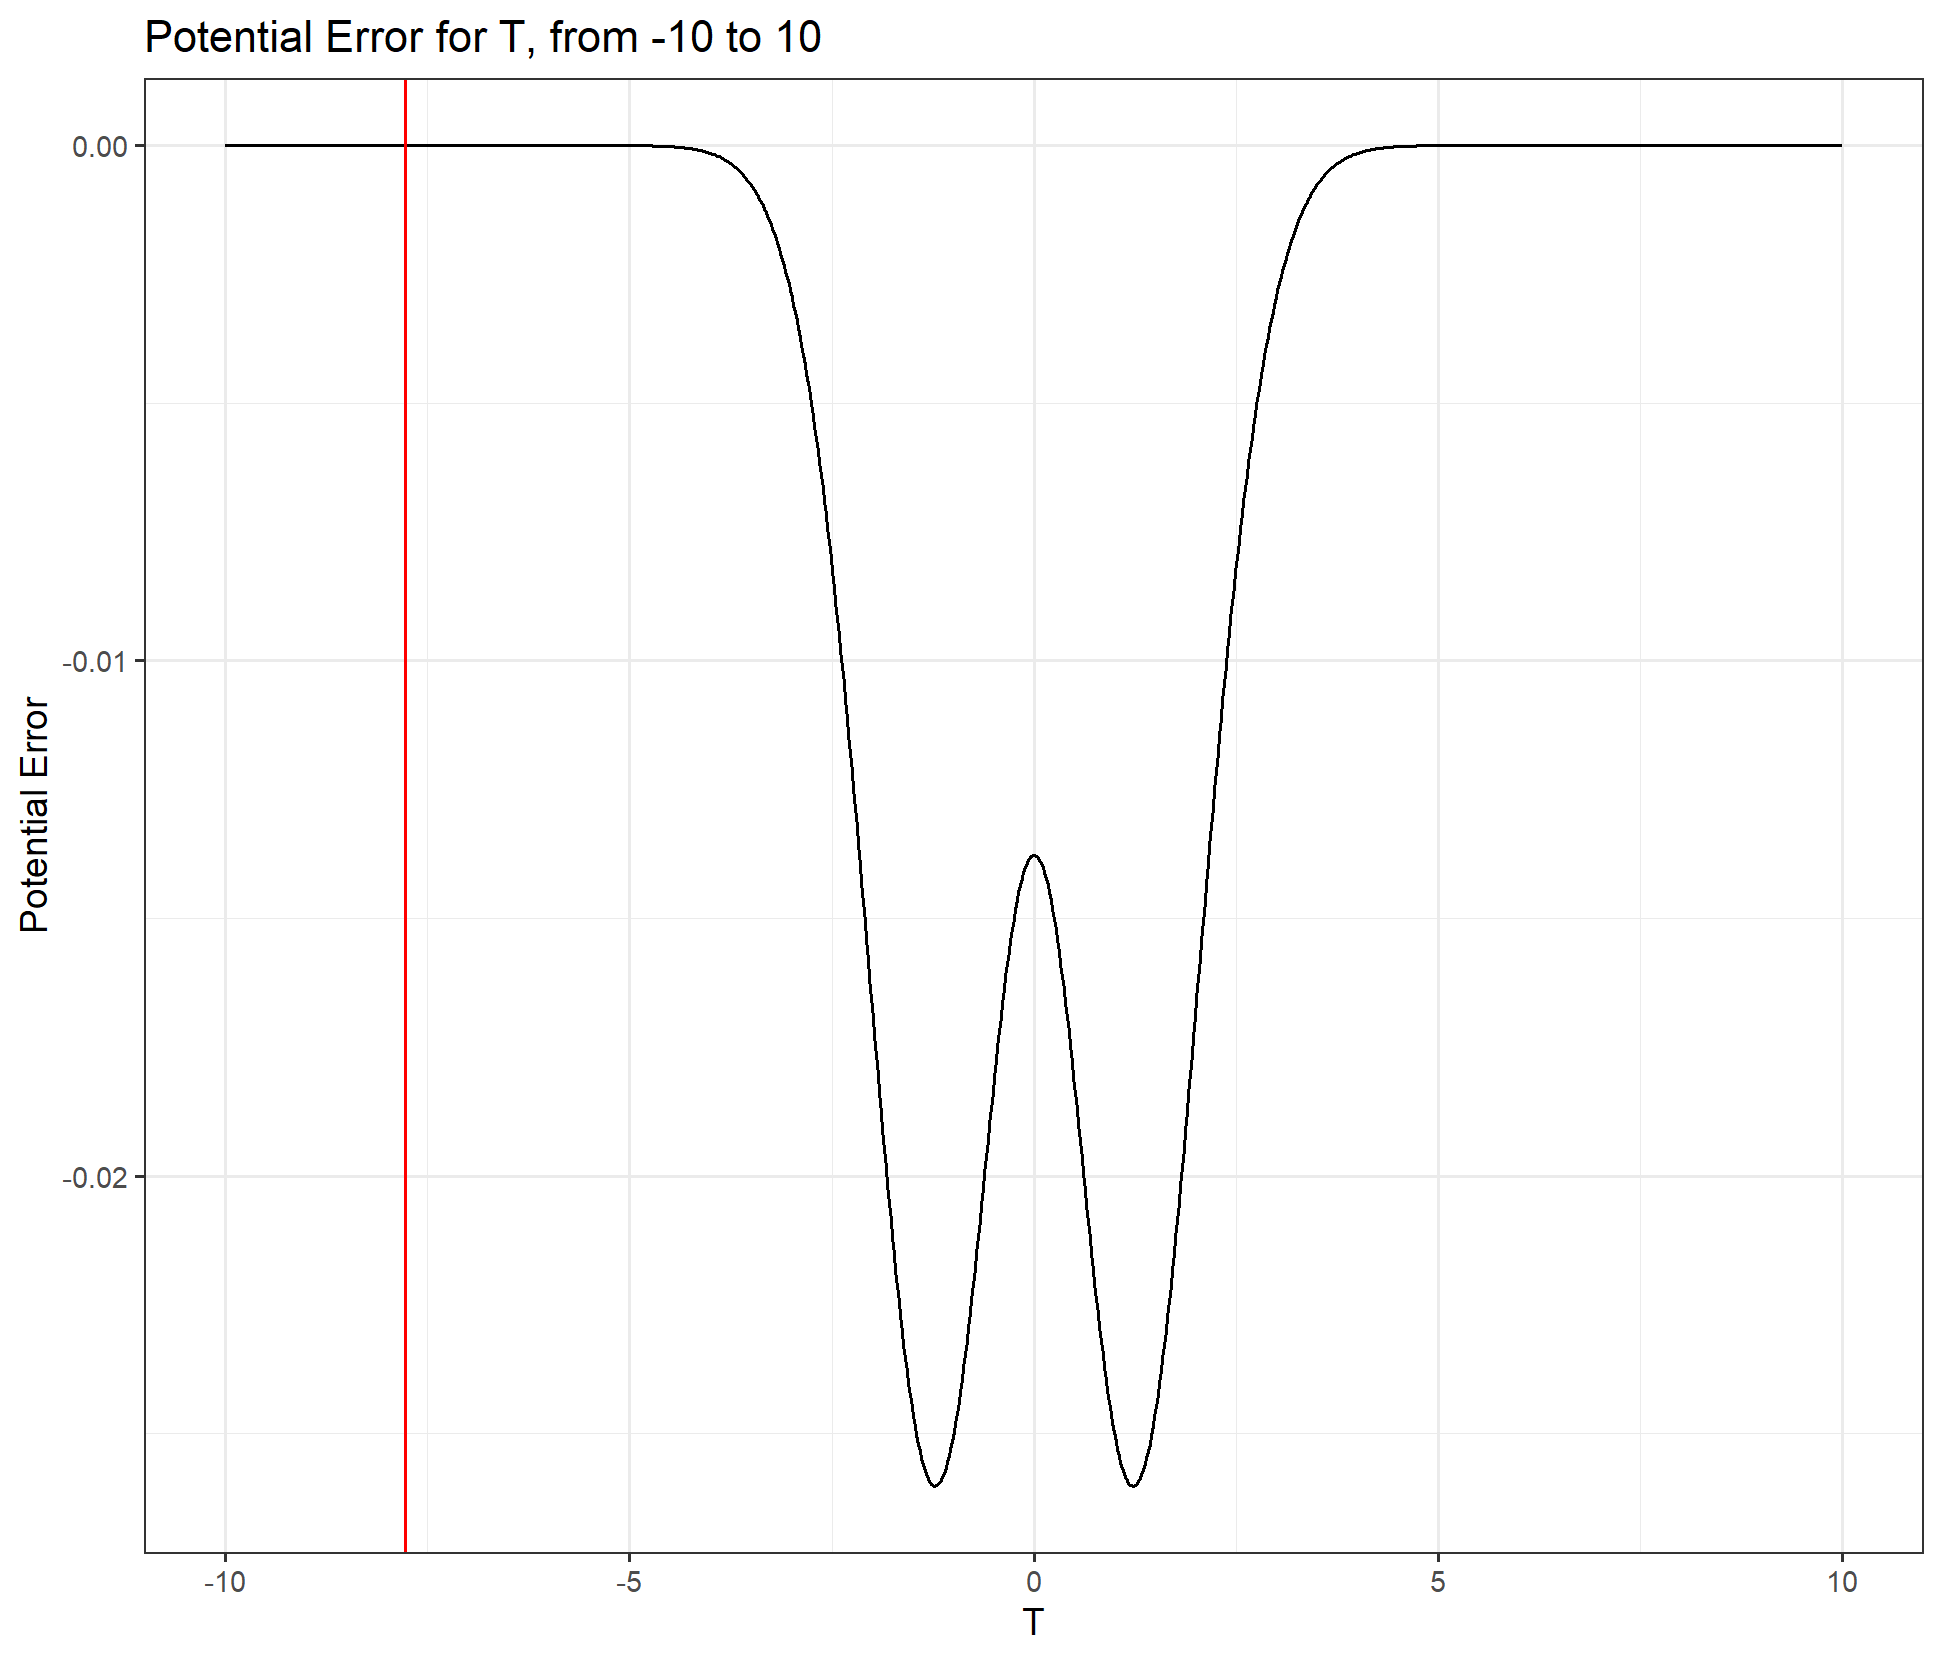
\includegraphics[width=10cm, height=8.5cm]{errorplot.png}
\caption{Potential error for t statistic ranging from -10 to 10, using the skewness of the zebra finch further data. The vertical line shows the t statistic for the zebra finch further data}
\label{plot1}
\end{figure}

  \textbf{Solution:} Figure \ref{plot1} plots the error for the t statistic, ranging from -10 to 10. The t statistic for the further data is -7.7779912, indicating an exceedingly small error (nearly $0$).
  
  \item Suppose we wanted to have a tail probability within 10\% of the desired
  $\alpha=0.05$. Recall we did a left-tailed test using the further data.
  How large of a sample size would we need? That is, we need
  to solve the error formula equal to 10\% of the desired left-tail probability:
  \[0.10 \alpha  \stackrel{set}{=} \underbrace{\frac{\text{skew}}{\sqrt{n}} \frac{(2t^2+1)}{6} f_Z(t)}_{\textrm{error}},\]
  which yields
  \[ n = \left(\frac{\text{skew}}{6(0.10\alpha)} (2t^2 + 1) f_Z(t)\right)^2.\]\\
\begin{knitrout}
\definecolor{shadecolor}{rgb}{0.969, 0.969, 0.969}\color{fgcolor}\begin{kframe}
\begin{alltt}
\hldef{alpha} \hlkwb{<-} \hlnum{0.05}
\hldef{t.alpha} \hlkwb{<-} \hlkwd{qnorm}\hldef{(alpha)}

\hldef{(min.nsize} \hlkwb{<-} \hldef{((}\hlkwd{skewness}\hldef{(further.data)} \hlopt{*} \hldef{(}\hlnum{2}\hlopt{*}\hldef{t.alpha}\hlopt{^}\hlnum{2} \hlopt{+} \hlnum{1}\hldef{)} \hlopt{*} \hlkwd{dnorm}\hldef{(t.alpha))}\hlopt{/}
               \hldef{(}\hlnum{6} \hlopt{*} \hlnum{0.1}\hlopt{*} \hldef{alpha))}\hlopt{^}\hlnum{2}\hldef{)}
\end{alltt}
\begin{verbatim}
## [1] 520.8876
\end{verbatim}
\end{kframe}
\end{knitrout}
\textbf{Solution:} The smallest sample size we would need to have a tail probability within 10\% of the desired $\alpha=0.05$ is 521. The experiment's $n = 25$ is significantly smaller than this. 
\end{enumerate}
%%%%%%%%%%%%%%%%%%%%%%%%%%%%%%%%%%%%%%%%%%%%%%%%%%%%%%%%%%%%%%%%%%%%%%%%%%%%%%%%
%%%%%%%%%%%%%%%%%%%%%%%%%%%%%%%%%%%%%%%%%%%%%%%%%%%%%%%%%%%%%%%%%%%%%%%%%%%%%%%%
% Question 3
%%%%%%%%%%%%%%%%%%%%%%%%%%%%%%%%%%%%%%%%%%%%%%%%%%%%%%%%%%%%%%%%%%%%%%%%%%%%%%%%
%%%%%%%%%%%%%%%%%%%%%%%%%%%%%%%%%%%%%%%%%%%%%%%%%%%%%%%%%%%%%%%%%%%%%%%%%%%%%%%%
\item Complete the following steps to revisit the analyses from lab 11 using the
bootstrap procedure.
\begin{enumerate}
\item Now, consider the zebra finch data. We do not know the generating distributions
for the closer, further, and difference data, so perform resampling to approximate the 
sampling distribution of the $T$ statistic:
  \[T = \frac{\bar{x}_r - 0}{s/\sqrt{n}},\]
  where $\bar{x}_r$ is the mean computed on the r$^{th}$ resample and $s$ is the
  sample standard deviation from the original samples. At the end, create an
  object called \texttt{resamples.null.closer}, for example, and store the 
  resamples shifted to ensure they are consistent with the null hypotheses at the average 
  (i.e., here ensure the shifted resamples are 0 on average, corresponding
  to $t=0$, for each case). \\
\begin{knitrout}
\definecolor{shadecolor}{rgb}{0.969, 0.969, 0.969}\color{fgcolor}\begin{kframe}
\begin{alltt}
\hlcom{# part a}
\hldef{R} \hlkwb{<-} \hlnum{1000}
\hlcom{# data}
\hldef{further.data} \hlkwb{<-} \hldef{zebrafinch.data}\hlopt{$}\hldef{further}
\hldef{closer.data} \hlkwb{<-} \hldef{zebrafinch.data}\hlopt{$}\hldef{closer}
\hldef{diff.data} \hlkwb{<-} \hldef{zebrafinch.data}\hlopt{$}\hldef{diff}
\hlcom{# set.seed() to make results reproducible}
\hlkwd{set.seed}\hldef{(}\hlnum{13345}\hldef{)}
\hlcom{# resampling}
\hldef{resamples} \hlkwb{<-} \hlkwd{tibble}\hldef{(}\hlkwc{resamps.further} \hldef{=}\hlkwd{rep}\hldef{(}\hlnum{NA}\hldef{, R),}
                  \hlkwc{resamps.closer} \hldef{=}\hlkwd{rep}\hldef{(}\hlnum{NA}\hldef{, R),}
                  \hlkwc{resamps.diff} \hldef{=}\hlkwd{rep}\hldef{(}\hlnum{NA}\hldef{, R))}
\hlkwa{for} \hldef{(i} \hlkwa{in} \hlnum{1}\hlopt{:}\hldef{R)\{}
\hlcom{# further}
\hldef{further.resample} \hlkwb{<-} \hlkwd{sample}\hldef{(}\hlkwc{x} \hldef{= further.data,}
                        \hlkwc{size}\hldef{=} \hlkwd{length}\hldef{(further.data),}
                        \hlkwc{replace} \hldef{= T)}
\hldef{resamples}\hlopt{$}\hldef{resamps.further[i]} \hlkwb{<-} \hldef{(}\hlkwd{mean}\hldef{(further.resample} \hlopt{-} \hldef{mu0))}\hlopt{/}
                                \hldef{(}\hlkwd{sd}\hldef{(further.data)}\hlopt{/}\hlkwd{sqrt}\hldef{(n))}

\hlcom{# closer}
\hldef{closer.resample} \hlkwb{<-} \hlkwd{sample}\hldef{(}\hlkwc{x} \hldef{= closer.data,}
                           \hlkwc{size}\hldef{=} \hlkwd{length}\hldef{(closer.data),}
                           \hlkwc{replace} \hldef{= T)}
\hldef{resamples}\hlopt{$}\hldef{resamps.closer[i]} \hlkwb{<-} \hldef{(}\hlkwd{mean}\hldef{(closer.resample} \hlopt{-} \hldef{mu0))}\hlopt{/}
                                \hldef{(}\hlkwd{sd}\hldef{(closer.data)}\hlopt{/}\hlkwd{sqrt}\hldef{(n))}

\hlcom{# diff}
\hldef{diff.resample} \hlkwb{<-} \hlkwd{sample}\hldef{(}\hlkwc{x} \hldef{= diff.data,}
                          \hlkwc{size}\hldef{=} \hlkwd{length}\hldef{(diff.data),}
                          \hlkwc{replace} \hldef{= T)}
\hldef{resamples}\hlopt{$}\hldef{resamps.diff[i]} \hlkwb{<-} \hldef{(}\hlkwd{mean}\hldef{(diff.resample} \hlopt{-} \hldef{mu0))}\hlopt{/}
                             \hldef{(}\hlkwd{sd}\hldef{(diff.data)}\hlopt{/}\hlkwd{sqrt}\hldef{(n))}
\hldef{\}}

\hlcom{# shifting data}
\hldef{resamples} \hlkwb{<-} \hldef{resamples |>}
 \hlkwd{mutate}\hldef{(}\hlkwc{resamps.further.null} \hldef{= resamps.further} \hlopt{-} \hlkwd{mean}\hldef{(resamps.further),}
      \hlkwc{resamps.closer.null} \hldef{= resamps.closer} \hlopt{-} \hlkwd{mean}\hldef{(resamps.closer),}
      \hlkwc{resamps.diff.null} \hldef{= resamps.diff} \hlopt{-} \hlkwd{mean}\hldef{(resamps.diff))}
\end{alltt}
\end{kframe}
\end{knitrout}
\textbf{Solution:} Above is the code using to conducting resampling for the t statistic for the zebra finch data. Since we did resampling on the t statistic, which we want to be centered at 0, we shift the resamples by simply subtracting the mean of all the resamples to center. \verb|set.seed()| was used to create reproducible results. 
  
  \item Compute the bootstrap $p$-value for each test using the shifted resamples. How do these compare to the $t$-test $p$-values? \\
\begin{knitrout}
\definecolor{shadecolor}{rgb}{0.969, 0.969, 0.969}\color{fgcolor}\begin{kframe}
\begin{alltt}
\hlcom{# part b }
\hldef{boot.pvals} \hlkwb{<-} \hldef{resamples |>}
\hlkwd{summarize}\hldef{(}\hlkwc{p.further} \hldef{=} \hlkwd{mean}\hldef{(resamps.further.null} \hlopt{<=} \hlkwd{mean}\hldef{(resamps.further)),}
          \hlkwc{p.closer} \hldef{=} \hlkwd{mean}\hldef{(resamps.closer.null} \hlopt{>=} \hlkwd{mean}\hldef{(resamps.closer)),}
          \hlkwc{p.low.diff} \hldef{=} \hlkwd{mean}\hldef{(resamps.diff.null} \hlopt{<= -}\hlkwd{mean}\hldef{(resamps.diff)),}
          \hlkwc{p.high.diff} \hldef{=} \hlkwd{mean}\hldef{(resamps.diff.null} \hlopt{>=} \hlkwd{mean}\hldef{(resamps.diff)),}
          \hlkwc{pdiff} \hldef{= p.low.diff} \hlopt{+} \hldef{p.high.diff)}

\hlcom{# p vals from t test}
\hlcom{# further}
\hldef{t.pval.further} \hlkwb{<-} \hlkwd{t.test}\hldef{(}\hlkwc{x}\hldef{=further.data,} \hlkwc{mu} \hldef{= mu0,} \hlkwc{alternative} \hldef{=} \hlsng{"less"}\hldef{)}\hlopt{$}\hldef{p.value}
\hlcom{# closer }
\hldef{t.pval.closer} \hlkwb{<-} \hlkwd{t.test}\hldef{(}\hlkwc{x}\hldef{=closer.data,} \hlkwc{mu} \hldef{= mu0,} \hlkwc{alternative} \hldef{=} \hlsng{"greater"}\hldef{)}\hlopt{$}\hldef{p.value}
\hlcom{# diff}
\hldef{t.pval.further} \hlkwb{<-} \hlkwd{t.test}\hldef{(}\hlkwc{x}\hldef{=diff.data,} \hlkwc{mu} \hldef{= mu0,} \hlkwc{alternative} \hldef{=} \hlsng{"two.sided"}\hldef{)}\hlopt{$}\hldef{p.value}

\hlcom{# creating table}
\hldef{all.pvals} \hlkwb{<-} \hlkwd{tibble}\hldef{(}\hlkwc{test} \hldef{=} \hlkwd{c}\hldef{(}\hlsng{"T-test"}\hldef{,} \hlsng{"Bootstrapping"}\hldef{),}
                  \hlkwc{p.further} \hldef{=} \hlkwd{c}\hldef{(t.pval.further,boot.pvals}\hlopt{$}\hldef{p.further),}
                  \hlkwc{p.closer} \hldef{=} \hlkwd{c}\hldef{(t.pval.closer, boot.pvals}\hlopt{$}\hldef{p.closer),}
                  \hlkwc{p.diff} \hldef{=} \hlkwd{c}\hldef{(t.pval.closer, boot.pvals}\hlopt{$}\hldef{pdiff))}

\hlkwd{xtable}\hldef{(all.pvals)}
\end{alltt}
\begin{verbatim}
## % latex table generated in R 4.4.2 by xtable 1.8-4 package
## % Fri May  2 14:31:24 2025
## \begin{table}[ht]
## \centering
## \begin{tabular}{rlrrr}
##   \hline
##  & test & p.further & p.closer & p.diff \\ 
##   \hline
## 1 & T-test & 0.00 & 0.00 & 0.00 \\ 
##   2 & Bootstrapping & 0.00 & 0.00 & 0.00 \\ 
##    \hline
## \end{tabular}
## \end{table}
\end{verbatim}
\end{kframe}
\end{knitrout}
\begin{table}[ht]
\centering
\begin{tabular}{rrrrr}
  \hline
 Type & p.further & p.closer & p.diff \\ 
  \hline
T-test & 0.00 & 0.00 & 0.00 \\ 
  Bootstrapping & 0.00 & 0.00 & 0.00 \\ 
   \hline
\end{tabular}
\caption{$p$-values for further, closer, and differences in the zebra finch data using the T-test and Bootstrapping}
\label{table1}
\end{table}
 \textbf{Solution:} The $p$-values calculated using bootstrapping is so small that it is effectively $0$ and treated as such, for the further, closer, and difference zebra finch data. In order to calculate the two-sided $p$-value for the difference data, you need to find the $p$-value on both tails, which can be found by adding or subtracting the mean of the difference data by $\delta$. However, since $\mu_0 = 0$, we can just using the negative of the mean of the difference data to get the ``mirror" observation on the other tail. $p$-values are compared in Table \ref{table1}.    
    \item What is the 5$^{th}$ percentile of the shifted resamples under the null hypothesis? 
  Note this value approximates $t_{0.05, n-1}$. Compare these values in each case. \\
\begin{knitrout}
\definecolor{shadecolor}{rgb}{0.969, 0.969, 0.969}\color{fgcolor}\begin{kframe}
\begin{alltt}
\hlcom{# part c}
\hlcom{# 5th percentile for t test (same for all)}
\hldef{t.5th} \hlkwb{<-} \hlkwd{qt}\hldef{(}\hlkwc{p}\hldef{=}\hlnum{0.05}\hldef{,} \hlkwc{df}\hldef{=n}\hlopt{-}\hlnum{1}\hldef{)}

\hlcom{# 5th percentile for bootstrapping }
\hlcom{# further}
\hldef{boot.f5th} \hlkwb{<-} \hlkwd{quantile}\hldef{(resamples}\hlopt{$}\hldef{resamps.further.null,} \hlnum{0.05}\hldef{)}

\hlcom{# closer}
\hldef{boot.c5th} \hlkwb{<-} \hlkwd{quantile}\hldef{(resamples}\hlopt{$}\hldef{resamps.closer.null,} \hlnum{0.05}\hldef{)}

\hlcom{# diff}
\hldef{boot.d5th} \hlkwb{<-} \hlkwd{quantile}\hldef{(resamples}\hlopt{$}\hldef{resamps.diff.null,} \hlnum{0.05}\hldef{)}

\hlcom{# create table}
\hldef{all.5thp} \hlkwb{<-} \hlkwd{tibble}\hldef{(}\hlkwc{Type} \hldef{=} \hlkwd{c}\hldef{(}\hlsng{"T-test"}\hldef{,} \hlsng{"Bootstrapping"}\hldef{),}
                 \hlkwc{further} \hldef{=} \hlkwd{c}\hldef{(t.5th, boot.f5th),}
                 \hlkwc{closer} \hldef{=} \hlkwd{c}\hldef{(t.5th, boot.c5th),}
                 \hlkwc{diff} \hldef{=} \hlkwd{c}\hldef{(t.5th, boot.d5th))}
\hlkwd{xtable}\hldef{(all.5thp)}
\end{alltt}
\begin{verbatim}
## % latex table generated in R 4.4.2 by xtable 1.8-4 package
## % Fri May  2 14:31:24 2025
## \begin{table}[ht]
## \centering
## \begin{tabular}{rlrrr}
##   \hline
##  & Type & further & closer & diff \\ 
##   \hline
## 1 & T-test & -1.71 & -1.71 & -1.71 \\ 
##   2 & Bootstrapping & -1.60 & -1.58 & -1.59 \\ 
##    \hline
## \end{tabular}
## \end{table}
\end{verbatim}
\end{kframe}
\end{knitrout}
\begin{table}[ht]
\centering
\begin{tabular}{rlrrr}
  \hline
 Type & further & closer & diff \\ 
  \hline
T-test & -1.71 & -1.71 & -1.71 \\ 
Bootstrapping & -1.60 & -1.58 & -1.59 \\ 
   \hline
\end{tabular}
\caption{5$^{th}$ percentile of the shifted resamples of the t statistic for further, closer, and difference data, compared to the t-test.}
\label{table2}
\end{table}
\textbf{Solution:} The 5$^{th}$ percentile for the t-test is the same for all three sets of data, as they are all drawn from the T distribution. The shifted resamples for the t statistic from bootstrapping was calculated for further, closer, and difference data, and the values are compared in Table \ref{table2}. Interestingly, all of the bootstrap values are larger than the T-test ones.
  \item Compute the bootstrap confidence intervals using the resamples. How do these 
  compare to the $t$-test confidence intervals? \\
\begin{knitrout}
\definecolor{shadecolor}{rgb}{0.969, 0.969, 0.969}\color{fgcolor}\begin{kframe}
\begin{alltt}
\hlcom{# part d}
\hlcom{# need to keep track of mean (xbar) now}
\hldef{further.xbars} \hlkwb{<-} \hlkwd{rep}\hldef{(}\hlnum{NA}\hldef{, R)}
\hldef{closer.xbars} \hlkwb{<-} \hlkwd{rep}\hldef{(}\hlnum{NA}\hldef{, R)}
\hldef{diff.xbars} \hlkwb{<-} \hlkwd{rep}\hldef{(}\hlnum{NA}\hldef{, R)}

\hlkwa{for} \hldef{(i} \hlkwa{in} \hlnum{1}\hlopt{:}\hldef{R)\{}
\hlcom{# further}
\hldef{further.resample} \hlkwb{<-} \hlkwd{sample}\hldef{(}\hlkwc{x} \hldef{= further.data,}
                           \hlkwc{size}\hldef{=} \hlkwd{length}\hldef{(further.data),}
                           \hlkwc{replace} \hldef{= T)}
\hldef{further.xbars[i]} \hlkwb{<-} \hlkwd{mean}\hldef{(further.resample)}

\hlcom{# closer}
\hldef{closer.resample} \hlkwb{<-} \hlkwd{sample}\hldef{(}\hlkwc{x} \hldef{= closer.data,}
                          \hlkwc{size}\hldef{=} \hlkwd{length}\hldef{(closer.data),}
                          \hlkwc{replace} \hldef{= T)}
\hldef{closer.xbars[i]} \hlkwb{<-} \hlkwd{mean}\hldef{(closer.resample)}

\hlcom{# diff}
\hldef{diff.resample} \hlkwb{<-} \hlkwd{sample}\hldef{(}\hlkwc{x} \hldef{= diff.data,}
                        \hlkwc{size}\hldef{=} \hlkwd{length}\hldef{(diff.data),}
                        \hlkwc{replace} \hldef{= T)}
\hldef{diff.xbars[i]} \hlkwb{<-} \hlkwd{mean}\hldef{(diff.resample)}
\hldef{\}}

\hlcom{# bca test}
\hlcom{# helper function}
\hldef{boot.mean} \hlkwb{<-} \hlkwa{function}\hldef{(}\hlkwc{d}\hldef{,} \hlkwc{i}\hldef{)\{}
\hlkwd{mean}\hldef{(d[i])}
\hldef{\}}
\hldef{R} \hlkwb{<-} \hlnum{1000}
\hlcom{# further}
\hldef{further.helper} \hlkwb{<-} \hlkwd{boot}\hldef{(}\hlkwc{data} \hldef{= further.data,}
                     \hlkwc{statistic} \hldef{= boot.mean,}
                     \hlkwc{R} \hldef{= R)}
\hlcom{# closer}
\hldef{closer.helper} \hlkwb{<-} \hlkwd{boot}\hldef{(}\hlkwc{data} \hldef{= closer.data,}
                    \hlkwc{statistic} \hldef{= boot.mean,}
                    \hlkwc{R} \hldef{= R)}
\hlcom{# diff}
\hldef{diff.helper} \hlkwb{<-} \hlkwd{boot}\hldef{(}\hlkwc{data} \hldef{= diff.data,}
                  \hlkwc{statistic} \hldef{= boot.mean,}
                  \hlkwc{R} \hldef{= R)}

\hlcom{# CI}
\hlcom{# further}
\hldef{(boot.further.CI} \hlkwb{<-} \hlkwd{quantile}\hldef{(further.xbars,} \hlkwd{c}\hldef{(}\hlnum{0.025}\hldef{,} \hlnum{0.975}\hldef{)))}
\end{alltt}
\begin{verbatim}
##       2.5%      97.5% 
## -0.2540837 -0.1601393
\end{verbatim}
\begin{alltt}
\hldef{(t.further.CI} \hlkwb{<-} \hlkwd{t.test}\hldef{(}\hlkwc{x}\hldef{=further.data,} \hlkwc{mu}\hldef{=mu0,} \hlkwc{alternative} \hldef{=} \hlsng{"two.sided"}\hldef{)}\hlopt{$}\hldef{conf.int)}
\end{alltt}
\begin{verbatim}
## [1] -0.2565176 -0.1489313
## attr(,"conf.level")
## [1] 0.95
\end{verbatim}
\begin{alltt}
\hldef{(further.bca} \hlkwb{<-} \hlkwd{boot.ci}\hldef{(further.helper,} \hlkwc{type}\hldef{=}\hlsng{"bca"}\hldef{))}
\end{alltt}
\begin{verbatim}
## BOOTSTRAP CONFIDENCE INTERVAL CALCULATIONS
## Based on 1000 bootstrap replicates
## 
## CALL : 
## boot.ci(boot.out = further.helper, type = "bca")
## 
## Intervals : 
## Level       BCa          
## 95%   (-0.2596, -0.1578 )  
## Calculations and Intervals on Original Scale
\end{verbatim}
\begin{alltt}
\hlcom{# closer}
\hldef{(boot.closer.CI} \hlkwb{<-} \hlkwd{quantile}\hldef{(closer.xbars,} \hlkwd{c}\hldef{(}\hlnum{0.025}\hldef{,} \hlnum{0.975}\hldef{)))}
\end{alltt}
\begin{verbatim}
##      2.5%     97.5% 
## 0.1244849 0.1926684
\end{verbatim}
\begin{alltt}
\hldef{(t.closer.CI} \hlkwb{<-} \hlkwd{t.test}\hldef{(}\hlkwc{x}\hldef{=closer.data,} \hlkwc{mu}\hldef{=mu0,} \hlkwc{alternative} \hldef{=} \hlsng{"two.sided"}\hldef{)}\hlopt{$}\hldef{conf.int)}
\end{alltt}
\begin{verbatim}
## [1] 0.1173875 0.1950586
## attr(,"conf.level")
## [1] 0.95
\end{verbatim}
\begin{alltt}
\hldef{(closer.bca} \hlkwb{<-} \hlkwd{boot.ci}\hldef{(closer.helper,} \hlkwc{type}\hldef{=}\hlsng{"bca"}\hldef{))}
\end{alltt}
\begin{verbatim}
## BOOTSTRAP CONFIDENCE INTERVAL CALCULATIONS
## Based on 1000 bootstrap replicates
## 
## CALL : 
## boot.ci(boot.out = closer.helper, type = "bca")
## 
## Intervals : 
## Level       BCa          
## 95%   ( 0.1218,  0.1920 )  
## Calculations and Intervals on Original Scale
\end{verbatim}
\begin{alltt}
\hlcom{# diff}
\hldef{(boot.diff.CI} \hlkwb{<-} \hlkwd{quantile}\hldef{(diff.xbars,} \hlkwd{c}\hldef{(}\hlnum{0.025}\hldef{,} \hlnum{0.975}\hldef{)))}
\end{alltt}
\begin{verbatim}
##      2.5%     97.5% 
## 0.2858302 0.4470153
\end{verbatim}
\begin{alltt}
\hldef{(t.diff.CI} \hlkwb{<-} \hlkwd{t.test}\hldef{(}\hlkwc{x}\hldef{=diff.data,} \hlkwc{mu}\hldef{=mu0,} \hlkwc{alternative} \hldef{=} \hlsng{"two.sided"}\hldef{)}\hlopt{$}\hldef{conf.int)}
\end{alltt}
\begin{verbatim}
## [1] 0.2719028 0.4459921
## attr(,"conf.level")
## [1] 0.95
\end{verbatim}
\begin{alltt}
\hldef{(diff.bca} \hlkwb{<-} \hlkwd{boot.ci}\hldef{(diff.helper,} \hlkwc{type}\hldef{=}\hlsng{"bca"}\hldef{))}
\end{alltt}
\begin{verbatim}
## BOOTSTRAP CONFIDENCE INTERVAL CALCULATIONS
## Based on 1000 bootstrap replicates
## 
## CALL : 
## boot.ci(boot.out = diff.helper, type = "bca")
## 
## Intervals : 
## Level       BCa          
## 95%   ( 0.2857,  0.4514 )  
## Calculations and Intervals on Original Scale
\end{verbatim}
\end{kframe}
\end{knitrout}
\textbf{Solution:} The $95\%$ confidence intervals for the further data are ($-0.254, -0.160$) using bootstrap percentile confidence interval, ($-0.260$, $-0.158$) using the bootstrap BCa, and ($-0.257, -0.149$) for the t-test.\\
The $95\%$ confidence intervals for the closer data are ($0.124, 0.193$) using bootstrap percentile confidence interval, ($0.122$, $0.192$) using the bootstrap BCa, and ($0.117, 0.195$) for the t-test. \\
The $95\%$ confidence intervals for the difference data are ($0.286, 0.447$) using bootstrap percentile confidence interval, ($0.286$, $0.451$) using the bootstrap BCa, and ($0.272, 0.446$) for the t-test. \\
Because the CIs were calculated on the data directly, we needed to conduct resampling again for each of the data's sample means instead of t-statistic. \\
The BCa confidence intervals and the percentile confidence intervals were very similar to each other, suggesting there is not much bias or skewness in the data. \\
Additionally, since $n=25$, we can assume that at least some sort of normality and symmetry emerges when conducting resampling, as its close to the boundary for CLT ($n=30$).
\end{enumerate}
%%%%%%%%%%%%%%%%%%%%%%%%%%%%%%%%%%%%%%%%%%%%%%%%%%%%%%%%%%%%%%%%%%%%%%%%%%%%%%%%
%%%%%%%%%%%%%%%%%%%%%%%%%%%%%%%%%%%%%%%%%%%%%%%%%%%%%%%%%%%%%%%%%%%%%%%%%%%%%%%%
% Question 4
%%%%%%%%%%%%%%%%%%%%%%%%%%%%%%%%%%%%%%%%%%%%%%%%%%%%%%%%%%%%%%%%%%%%%%%%%%%%%%%%
%%%%%%%%%%%%%%%%%%%%%%%%%%%%%%%%%%%%%%%%%%%%%%%%%%%%%%%%%%%%%%%%%%%%%%%%%%%%%%%%
\item Complete the following steps to revisit the analyses from lab 11 using the
randomization procedure.
\begin{enumerate}
\item Now, consider the zebra finch data. We do not know the generating distributions
for the closer, further, and difference data, so perform the randomization procedure. \\
\begin{knitrout}
\definecolor{shadecolor}{rgb}{0.969, 0.969, 0.969}\color{fgcolor}\begin{kframe}
\begin{alltt}
\hlcom{# part a}
\hlkwd{set.seed}\hldef{(}\hlnum{13345}\hldef{)}
\hldef{R} \hlkwb{<-} \hlnum{1000}
\hldef{rand} \hlkwb{<-} \hlkwd{tibble}\hldef{(}\hlkwc{xbars.further} \hldef{=} \hlkwd{rep}\hldef{(}\hlnum{NA}\hldef{, R),}
               \hlkwc{xbars.closer} \hldef{=} \hlkwd{rep}\hldef{(}\hlnum{NA}\hldef{, R),}
               \hlkwc{xbars.diff} \hldef{=} \hlkwd{rep}\hldef{(}\hlnum{NA}\hldef{, R))}
\hlcom{# since mean 0 (mu0 = 0) under H0 is given, no need to shift}

\hlcom{# RANDOMIZE / SHUFFLE}
\hlkwa{for}\hldef{(i} \hlkwa{in} \hlnum{1}\hlopt{:}\hldef{R)\{}
  \hlcom{# further}
  \hldef{further.rand} \hlkwb{<-} \hldef{further.data} \hlopt{*}
    \hlkwd{sample}\hldef{(}\hlkwc{x} \hldef{=} \hlkwd{c}\hldef{(}\hlopt{-}\hlnum{1}\hldef{,} \hlnum{1}\hldef{),}
           \hlkwc{size} \hldef{=} \hlkwd{length}\hldef{(further.data),}
           \hlkwc{replace} \hldef{= T)}

  \hldef{rand}\hlopt{$}\hldef{xbars.further[i]} \hlkwb{<-} \hlkwd{mean}\hldef{(further.rand)}

  \hlcom{# closer}
  \hldef{closer.rand} \hlkwb{<-} \hldef{closer.data} \hlopt{*}
    \hlkwd{sample}\hldef{(}\hlkwc{x} \hldef{=} \hlkwd{c}\hldef{(}\hlopt{-}\hlnum{1}\hldef{,} \hlnum{1}\hldef{),}
           \hlkwc{size} \hldef{=} \hlkwd{length}\hldef{(closer.data),}
           \hlkwc{replace} \hldef{= T)}

  \hldef{rand}\hlopt{$}\hldef{xbars.closer[i]} \hlkwb{<-} \hlkwd{mean}\hldef{(closer.rand)}

  \hlcom{# diff}
  \hldef{diff.rand} \hlkwb{<-} \hldef{diff.data} \hlopt{*}
    \hlkwd{sample}\hldef{(}\hlkwc{x} \hldef{=} \hlkwd{c}\hldef{(}\hlopt{-}\hlnum{1}\hldef{,} \hlnum{1}\hldef{),}
           \hlkwc{size} \hldef{=} \hlkwd{length}\hldef{(diff.data),}
           \hlkwc{replace} \hldef{= T)}

  \hldef{rand}\hlopt{$}\hldef{xbars.diff[i]} \hlkwb{<-} \hlkwd{mean}\hldef{(diff.rand)}
\hldef{\}}

\hlcom{# no need to shift back either!}
\end{alltt}
\end{kframe}
\end{knitrout}
\textbf{Solution:} The procedure for the randomization test is conducted in the code above. However, because our $H_0$ is specified as $\mu = 0$, we do not need to shift the data before and after shuffling because its already centered around $0$. 
  \item Compute the randomization test $p$-value for each test. \\
\begin{knitrout}
\definecolor{shadecolor}{rgb}{0.969, 0.969, 0.969}\color{fgcolor}\begin{kframe}
\begin{alltt}
\hlcom{# task b}
\hlcom{# p-value }
\hldef{(rand.pvals} \hlkwb{<-} \hldef{rand |>}
\hlkwd{summarize}\hldef{(}\hlkwc{p.further} \hldef{=} \hlkwd{mean}\hldef{(xbars.further} \hlopt{<=} \hlkwd{mean}\hldef{(further.data)),}
          \hlkwc{p.closer} \hldef{=} \hlkwd{mean}\hldef{(xbars.closer} \hlopt{>=} \hlkwd{mean}\hldef{(closer.data)),}
          \hlkwc{p.low.diff} \hldef{=} \hlkwd{mean}\hldef{(xbars.diff} \hlopt{<= -}\hlkwd{mean}\hldef{(diff.data)),}
          \hlkwc{p.high.diff} \hldef{=} \hlkwd{mean}\hldef{(xbars.diff} \hlopt{>=} \hlkwd{mean}\hldef{(diff.data)),}
          \hlkwc{pdiff} \hldef{= p.low.diff} \hlopt{+} \hldef{p.high.diff))}
\end{alltt}
\begin{verbatim}
## # A tibble: 1 x 5
##   p.further p.closer p.low.diff p.high.diff pdiff
##       <dbl>    <dbl>      <dbl>       <dbl> <dbl>
## 1         0        0          0           0     0
\end{verbatim}
\end{kframe}
\end{knitrout}
\begin{table}[ht]
\centering
\begin{tabular}{rrrrr}
  \hline
 Type & p.further & p.closer & p.diff \\ 
  \hline
T-test & 0.00 & 0.00 & 0.00 \\ 
  Bootstrapping & 0.00 & 0.00 & 0.00 \\
  Randomization & 0.00 & 0.00 & 0.00 \\
   \hline
\end{tabular}
\caption{$p$-values for further, closer, and differences in the zebra finch data using the T-test, Bootstrapping, and Randomization}
\label{table3}
\end{table}
  \textbf{Solution:} Similar to the bootstrap $p$-values, the values are so small that it is effectively $0$ across all the data. The randomization $p$-value procedure is nearly identical to the bootstrap $p$-value, except we are now comparing shifted resampled means to the sample mean. $p$-values are compared in Table \ref{table3}.
  
  \item Compute the randomization confidence interval by iterating over values of $\mu_0$.\\
  \textbf{Hint:} You can ``search" for the lower bound from $Q_1$ and subtracting by 0.0001, 
  and the upper bound using $Q_3$ and increasing by 0.0001. You will continue until you find 
  the first value for which the two-sided $p$-value is greater than or equal to 0.05. \\
\begin{knitrout}
\definecolor{shadecolor}{rgb}{0.969, 0.969, 0.969}\color{fgcolor}\begin{kframe}
\begin{alltt}
\hlcom{# task c}
\hlcom{# further }
\hldef{R} \hlkwb{<-} \hlnum{1000}
\hldef{mu0.iterate.further} \hlkwb{<-} \hlnum{0.01}
\hldef{starting.point.further} \hlkwb{<-} \hlkwd{mean}\hldef{(further.data)}

\hldef{mu.lower.further} \hlkwb{<-} \hldef{starting.point.further}
\hlkwa{repeat}\hldef{\{}
\hldef{rand} \hlkwb{<-} \hlkwd{tibble}\hldef{(}\hlkwc{xbars} \hldef{=} \hlkwd{rep}\hldef{(}\hlnum{NA}\hldef{, R))}

\hlcom{# PREPROCESSING: shift the data to be mean 0 under H0}
\hldef{x.shift} \hlkwb{<-} \hldef{further.data} \hlopt{-} \hldef{mu.lower.further}
\hlcom{# RANDOMIZE / SHUFFLE}
\hlkwa{for}\hldef{(i} \hlkwa{in} \hlnum{1}\hlopt{:}\hldef{R)\{}
  \hldef{curr.rand} \hlkwb{<-} \hldef{x.shift} \hlopt{*}
    \hlkwd{sample}\hldef{(}\hlkwc{x} \hldef{=} \hlkwd{c}\hldef{(}\hlopt{-}\hlnum{1}\hldef{,} \hlnum{1}\hldef{),}
           \hlkwc{size} \hldef{=} \hlkwd{length}\hldef{(x.shift),}
           \hlkwc{replace} \hldef{= T)}

  \hldef{rand}\hlopt{$}\hldef{xbars[i]} \hlkwb{<-} \hlkwd{mean}\hldef{(curr.rand)}
\hldef{\}}
\hlcom{# Thinking is hard}
\hldef{rand} \hlkwb{<-} \hldef{rand |>}
  \hlkwd{mutate}\hldef{(}\hlkwc{xbars} \hldef{= xbars} \hlopt{+} \hldef{mu.lower.further)} \hlcom{# shifting back}

\hlcom{# p-value }
\hldef{p.val} \hlkwb{<-}\hlkwd{mean}\hldef{(rand}\hlopt{$}\hldef{xbars} \hlopt{>=} \hlkwd{mean}\hldef{(further.data))}

\hlkwa{if}\hldef{(p.val} \hlopt{<} \hlnum{0.05}\hldef{)\{}
  \hlkwa{break}
\hldef{\}}\hlkwa{else}\hldef{\{}
  \hldef{mu.lower.further} \hlkwb{<-} \hldef{mu.lower.further} \hlopt{-} \hldef{mu0.iterate.further}
\hldef{\}}
\hldef{\}}

\hldef{mu.upper.further} \hlkwb{<-} \hldef{starting.point.further}
\hlkwa{repeat}\hldef{\{}
\hldef{rand} \hlkwb{<-} \hlkwd{tibble}\hldef{(}\hlkwc{xbars} \hldef{=} \hlkwd{rep}\hldef{(}\hlnum{NA}\hldef{, R))}

\hlcom{# PREPROCESSING: shift the data to be mean 0 under H0}
\hldef{x.shift} \hlkwb{<-} \hldef{further.data} \hlopt{-} \hldef{mu.upper.further}
\hlcom{# RANDOMIZE / SHUFFLE}
\hlkwa{for}\hldef{(i} \hlkwa{in} \hlnum{1}\hlopt{:}\hldef{R)\{}
  \hldef{curr.rand} \hlkwb{<-} \hldef{x.shift} \hlopt{*}
    \hlkwd{sample}\hldef{(}\hlkwc{x} \hldef{=} \hlkwd{c}\hldef{(}\hlopt{-}\hlnum{1}\hldef{,} \hlnum{1}\hldef{),}
           \hlkwc{size} \hldef{=} \hlkwd{length}\hldef{(x.shift),}
           \hlkwc{replace} \hldef{= T)}

  \hldef{rand}\hlopt{$}\hldef{xbars[i]} \hlkwb{<-} \hlkwd{mean}\hldef{(curr.rand)}
\hldef{\}}
\hlcom{# Thinking is hard}
\hldef{rand} \hlkwb{<-} \hldef{rand |>}
  \hlkwd{mutate}\hldef{(}\hlkwc{xbars} \hldef{= xbars} \hlopt{+} \hldef{mu.upper.further)} \hlcom{# shifting back}

\hlcom{# p-value }
\hldef{p.val} \hlkwb{<-}\hlkwd{mean}\hldef{(rand}\hlopt{$}\hldef{xbars} \hlopt{<=} \hlkwd{mean}\hldef{(further.data))}

\hlkwa{if}\hldef{(p.val} \hlopt{<} \hlnum{0.05}\hldef{)\{}
  \hlkwa{break}
\hldef{\}}\hlkwa{else}\hldef{\{}
  \hldef{mu.upper.further} \hlkwb{<-} \hldef{mu.upper.further} \hlopt{+} \hldef{mu0.iterate.further}
\hldef{\}}
\hldef{\}}

\hlkwd{c}\hldef{(mu.lower.further, mu.upper.further)}
\end{alltt}
\begin{verbatim}
## [1] -0.2527244 -0.1527244
\end{verbatim}
\begin{alltt}
\hlcom{# closer}
\hldef{R} \hlkwb{<-} \hlnum{1000}
\hldef{mu0.iterate.closer} \hlkwb{<-} \hlnum{0.01}
\hldef{starting.point.closer} \hlkwb{<-} \hlkwd{mean}\hldef{(closer.data)}

\hldef{mu.lower.closer} \hlkwb{<-} \hldef{starting.point.closer}
\hlkwa{repeat}\hldef{\{}
\hldef{rand} \hlkwb{<-} \hlkwd{tibble}\hldef{(}\hlkwc{xbars} \hldef{=} \hlkwd{rep}\hldef{(}\hlnum{NA}\hldef{, R))}

\hlcom{# PREPROCESSING: shift the data to be mean 0 under H0}
\hldef{x.shift} \hlkwb{<-} \hldef{closer.data} \hlopt{-} \hldef{mu.lower.closer}
\hlcom{# RANDOMIZE / SHUFFLE}
\hlkwa{for}\hldef{(i} \hlkwa{in} \hlnum{1}\hlopt{:}\hldef{R)\{}
  \hldef{curr.rand} \hlkwb{<-} \hldef{x.shift} \hlopt{*}
    \hlkwd{sample}\hldef{(}\hlkwc{x} \hldef{=} \hlkwd{c}\hldef{(}\hlopt{-}\hlnum{1}\hldef{,} \hlnum{1}\hldef{),}
           \hlkwc{size} \hldef{=} \hlkwd{length}\hldef{(x.shift),}
           \hlkwc{replace} \hldef{= T)}

  \hldef{rand}\hlopt{$}\hldef{xbars[i]} \hlkwb{<-} \hlkwd{mean}\hldef{(curr.rand)}
\hldef{\}}
\hlcom{# Thinking is hard}
\hldef{rand} \hlkwb{<-} \hldef{rand |>}
  \hlkwd{mutate}\hldef{(}\hlkwc{xbars} \hldef{= xbars} \hlopt{+} \hldef{mu.lower.closer)} \hlcom{# shifting back}

\hlcom{# p-value }
\hldef{p.val} \hlkwb{<-}\hlkwd{mean}\hldef{(rand}\hlopt{$}\hldef{xbars} \hlopt{>=} \hlkwd{mean}\hldef{(closer.data))}

\hlkwa{if}\hldef{(p.val} \hlopt{<} \hlnum{0.05}\hldef{)\{}
  \hlkwa{break}
\hldef{\}}\hlkwa{else}\hldef{\{}
  \hldef{mu.lower.closer} \hlkwb{<-} \hldef{mu.lower.closer} \hlopt{-} \hldef{mu0.iterate.closer}
\hldef{\}}
\hldef{\}}

\hldef{mu.upper.closer} \hlkwb{<-} \hldef{starting.point.closer}
\hlkwa{repeat}\hldef{\{}
\hldef{rand} \hlkwb{<-} \hlkwd{tibble}\hldef{(}\hlkwc{xbars} \hldef{=} \hlkwd{rep}\hldef{(}\hlnum{NA}\hldef{, R))}

\hlcom{# PREPROCESSING: shift the data to be mean 0 under H0}
\hldef{x.shift} \hlkwb{<-} \hldef{closer.data} \hlopt{-} \hldef{mu.upper.closer}
\hlcom{# RANDOMIZE / SHUFFLE}
\hlkwa{for}\hldef{(i} \hlkwa{in} \hlnum{1}\hlopt{:}\hldef{R)\{}
  \hldef{curr.rand} \hlkwb{<-} \hldef{x.shift} \hlopt{*}
    \hlkwd{sample}\hldef{(}\hlkwc{x} \hldef{=} \hlkwd{c}\hldef{(}\hlopt{-}\hlnum{1}\hldef{,} \hlnum{1}\hldef{),}
           \hlkwc{size} \hldef{=} \hlkwd{length}\hldef{(x.shift),}
           \hlkwc{replace} \hldef{= T)}

  \hldef{rand}\hlopt{$}\hldef{xbars[i]} \hlkwb{<-} \hlkwd{mean}\hldef{(curr.rand)}
\hldef{\}}
\hlcom{# Thinking is hard}
\hldef{rand} \hlkwb{<-} \hldef{rand |>}
  \hlkwd{mutate}\hldef{(}\hlkwc{xbars} \hldef{= xbars} \hlopt{+} \hldef{mu.upper.closer)} \hlcom{# shifting back}

\hlcom{# p-value }
\hldef{p.val} \hlkwb{<-}\hlkwd{mean}\hldef{(rand}\hlopt{$}\hldef{xbars} \hlopt{<=} \hlkwd{mean}\hldef{(closer.data))}

\hlkwa{if}\hldef{(p.val} \hlopt{<} \hlnum{0.05}\hldef{)\{}
  \hlkwa{break}
\hldef{\}}\hlkwa{else}\hldef{\{}
  \hldef{mu.upper.closer} \hlkwb{<-} \hldef{mu.upper.closer} \hlopt{+} \hldef{mu0.iterate.closer}
\hldef{\}}
\hldef{\}}

\hlkwd{c}\hldef{(mu.lower.closer, mu.upper.closer)}
\end{alltt}
\begin{verbatim}
## [1] 0.1162231 0.1962231
\end{verbatim}
\begin{alltt}
\hlcom{# diff}
\hldef{R} \hlkwb{<-} \hlnum{1000}
\hldef{mu0.iterate.diff} \hlkwb{<-} \hlnum{0.01}
\hldef{starting.point.diff} \hlkwb{<-} \hlkwd{mean}\hldef{(diff.data)}

\hldef{mu.lower.diff} \hlkwb{<-} \hldef{starting.point.diff}
\hlkwa{repeat}\hldef{\{}
\hldef{rand} \hlkwb{<-} \hlkwd{tibble}\hldef{(}\hlkwc{xbars} \hldef{=} \hlkwd{rep}\hldef{(}\hlnum{NA}\hldef{, R))}

\hlcom{# PREPROCESSING: shift the data to be mean 0 under H0}
\hldef{x.shift} \hlkwb{<-} \hldef{diff.data} \hlopt{-} \hldef{mu.lower.diff}
\hlcom{# RANDOMIZE / SHUFFLE}
\hlkwa{for}\hldef{(i} \hlkwa{in} \hlnum{1}\hlopt{:}\hldef{R)\{}
  \hldef{curr.rand} \hlkwb{<-} \hldef{x.shift} \hlopt{*}
    \hlkwd{sample}\hldef{(}\hlkwc{x} \hldef{=} \hlkwd{c}\hldef{(}\hlopt{-}\hlnum{1}\hldef{,} \hlnum{1}\hldef{),}
           \hlkwc{size} \hldef{=} \hlkwd{length}\hldef{(x.shift),}
           \hlkwc{replace} \hldef{= T)}

  \hldef{rand}\hlopt{$}\hldef{xbars[i]} \hlkwb{<-} \hlkwd{mean}\hldef{(curr.rand)}
\hldef{\}}
\hlcom{# Thinking is hard}
\hldef{rand} \hlkwb{<-} \hldef{rand |>}
  \hlkwd{mutate}\hldef{(}\hlkwc{xbars} \hldef{= xbars} \hlopt{+} \hldef{mu.lower.diff)} \hlcom{# shifting back}

\hlcom{# p-value }
\hldef{delta} \hlkwb{<-} \hlkwd{abs}\hldef{(}\hlkwd{mean}\hldef{(diff.data)} \hlopt{-} \hldef{mu.lower.diff)}
\hldef{low} \hlkwb{<-} \hldef{mu.lower.diff} \hlopt{-} \hldef{delta} \hlcom{# mirror}
\hldef{high} \hlkwb{<-} \hldef{mu.lower.diff} \hlopt{+} \hldef{delta}   \hlcom{# xbar}
\hldef{p.val} \hlkwb{<-} \hlkwd{mean}\hldef{(rand}\hlopt{$}\hldef{xbars} \hlopt{<=} \hldef{low)} \hlopt{+}
    \hlkwd{mean}\hldef{(rand}\hlopt{$}\hldef{xbars} \hlopt{>=} \hldef{high)}

\hlkwa{if}\hldef{(p.val} \hlopt{<} \hlnum{0.05}\hldef{)\{}
  \hlkwa{break}
\hldef{\}}\hlkwa{else}\hldef{\{}
  \hldef{mu.lower.diff} \hlkwb{<-} \hldef{mu.lower.diff} \hlopt{-} \hldef{mu0.iterate.diff}
\hldef{\}}
\hldef{\}}

\hldef{mu.upper.diff} \hlkwb{<-} \hldef{starting.point.diff}
\hlkwa{repeat}\hldef{\{}
\hldef{rand} \hlkwb{<-} \hlkwd{tibble}\hldef{(}\hlkwc{xbars} \hldef{=} \hlkwd{rep}\hldef{(}\hlnum{NA}\hldef{, R))}

\hlcom{# PREPROCESSING: shift the data to be mean 0 under H0}
\hldef{x.shift} \hlkwb{<-} \hldef{diff.data} \hlopt{-} \hldef{mu.upper.diff}
\hlcom{# RANDOMIZE / SHUFFLE}
\hlkwa{for}\hldef{(i} \hlkwa{in} \hlnum{1}\hlopt{:}\hldef{R)\{}
  \hldef{curr.rand} \hlkwb{<-} \hldef{x.shift} \hlopt{*}
    \hlkwd{sample}\hldef{(}\hlkwc{x} \hldef{=} \hlkwd{c}\hldef{(}\hlopt{-}\hlnum{1}\hldef{,} \hlnum{1}\hldef{),}
           \hlkwc{size} \hldef{=} \hlkwd{length}\hldef{(x.shift),}
           \hlkwc{replace} \hldef{= T)}

  \hldef{rand}\hlopt{$}\hldef{xbars[i]} \hlkwb{<-} \hlkwd{mean}\hldef{(curr.rand)}
\hldef{\}}
\hlcom{# Thinking is hard}
\hldef{rand} \hlkwb{<-} \hldef{rand |>}
  \hlkwd{mutate}\hldef{(}\hlkwc{xbars} \hldef{= xbars} \hlopt{+} \hldef{mu.upper.diff)} \hlcom{# shifting back}

\hlcom{# p-value }
\hldef{delta} \hlkwb{<-} \hlkwd{abs}\hldef{(}\hlkwd{mean}\hldef{(diff.data)} \hlopt{-} \hldef{mu.upper.diff)}
\hldef{low} \hlkwb{<-} \hldef{mu.upper.diff} \hlopt{-} \hldef{delta} \hlcom{# mirror}
\hldef{high} \hlkwb{<-} \hldef{mu.upper.diff} \hlopt{+} \hldef{delta}   \hlcom{# xbar}
\hldef{p.val} \hlkwb{<-} \hlkwd{mean}\hldef{(rand}\hlopt{$}\hldef{xbars} \hlopt{<=} \hldef{low)} \hlopt{+}
  \hlkwd{mean}\hldef{(rand}\hlopt{$}\hldef{xbars} \hlopt{>=} \hldef{high)}

\hlkwa{if}\hldef{(p.val} \hlopt{<} \hlnum{0.05}\hldef{)\{}
  \hlkwa{break}
\hldef{\}}\hlkwa{else}\hldef{\{}
  \hldef{mu.upper.diff} \hlkwb{<-} \hldef{mu.upper.diff} \hlopt{+} \hldef{mu0.iterate.diff}
\hldef{\}}
\hldef{\}}

\hlkwd{c}\hldef{(mu.lower.diff, mu.upper.diff)}
\end{alltt}
\begin{verbatim}
## [1] 0.2689475 0.4489475
\end{verbatim}
\end{kframe}
\end{knitrout}
  \textbf{Solution:} The $95\%$ randomization confidence intervals for the further data is ($-0.253$, $-0.153$), compared to the t-test ($-0.257$,$-0.149$), the bootstrap BCa ($-0.260$, $-0.158$), and the bootstrap percentile ($-0.254, -0.160$).\\
  The $95\%$ randomization confidence intervals for the closer data is ($0.116$, $0.196$), compared to the t-test ($0.117, 0.195$, the bootstrap BCa ($0.122$, $0.192$), and the bootstrap percentile ($0.124, 0.193$).\\
  The $95\%$ randomization confidence intervals for the difference data is ($0.269$, $0.449$), compared to the t-test ($0.272, 0.446$), the bootstrap Bca ($0.286$, $0.451$), and the bootstrap percentile ($0.286, 0.447$). \\
  As we can see, the confidence intervals for all the data using randomization is similar to the confidence intervals from the t-test and bootstrapping, which should make sense. \texttt{xbars} needs to be shifted when calculating the confidence interval because \verb|mu.lower| and \verb|mu.upper| change as we loop through to check. The randomization confidence interval is a lot more ``brute force" compared to the others, and we have to search over a grid manually to find the them. While we have historically used \verb|R <- 10000| in randomization, I switched to \verb|R <- 1000| so the code runs quicker.  
\end{enumerate}
%%%%%%%%%%%%%%%%%%%%%%%%%%%%%%%%%%%%%%%%%%%%%%%%%%%%%%%%%%%%%%%%%%%%%%%%%%%%%%%%
%%%%%%%%%%%%%%%%%%%%%%%%%%%%%%%%%%%%%%%%%%%%%%%%%%%%%%%%%%%%%%%%%%%%%%%%%%%%%%%%
% Optional Question
%%%%%%%%%%%%%%%%%%%%%%%%%%%%%%%%%%%%%%%%%%%%%%%%%%%%%%%%%%%%%%%%%%%%%%%%%%%%%%%%
%%%%%%%%%%%%%%%%%%%%%%%%%%%%%%%%%%%%%%%%%%%%%%%%%%%%%%%%%%%%%%%%%%%%%%%%%%%%%%%%
\item \textbf{Optional Challenge:} In this lab, you performed resampling to 
approximate the sampling distribution of the $T$ statistic using
\[T = \frac{\bar{x}_r - 0}{s/\sqrt{n}}.\]
I'm curious whether it is better/worse/similar if we computed the statistics
using the sample standard deviation of the resamples ($s_r$), instead of the 
original sample ($s$)
  \[T = \frac{\bar{x}_r - 0}{s_r/\sqrt{n}}.\]
\begin{enumerate}
  \item Perform a simulation study to evaluate the Type I error for conducting this
hypothesis test both ways.
  \item Using the same test case(s) as part (a), compute bootstrap confidence 
  intervals and assess their coverage -- how often do we `capture' the parameter
of interest?
\end{enumerate}
%%%%%%%%%%%%%%%%%%%%%%%%%%%%%%%%%%%%%%%%%%%%%%%%%%%%%%%%%%%%%%%%%%%%%%%%%%%%%%%%
%%%%%%%%%%%%%%%%%%%%%%%%%%%%%%%%%%%%%%%%%%%%%%%%%%%%%%%%%%%%%%%%%%%%%%%%%%%%%%%%
% End Document
%%%%%%%%%%%%%%%%%%%%%%%%%%%%%%%%%%%%%%%%%%%%%%%%%%%%%%%%%%%%%%%%%%%%%%%%%%%%%%%%
%%%%%%%%%%%%%%%%%%%%%%%%%%%%%%%%%%%%%%%%%%%%%%%%%%%%%%%%%%%%%%%%%%%%%%%%%%%%%%%%
\end{enumerate}
\bibliography{bibliography}
\end{document}

